\chapter{we hope you like typing} 
\label{sec:listing}
\lstset{style=6502Style}
Gather round children and let me tell you about a time when kids not unlike you were
so determined to see colors on a screen that they were prepared to spend hours punching
numbers into a computer terminal with only the very slim prospect that their efforts would not be utterly 
in vain.

This strange phenonemon was known as a 'listing'. Print magazines of the 1980s would run long lists of 
computer code for their apparently willing, and presumably adolescent, customers to type in to their home computers on the promise of
hours of fun. In an era that preceded widespread, practically-free forms of distribution such as the internet and
where purchasing a game on cassette or disk could run to as much as 60 pounds sterling,
this was an inexpensive way to obtain something resembling a computer game at a bargain price - paying for the pleasure
only at the expense of free time and patience.  

Prior to the release of Psychedelia in the Christmas of 1984, Jeff Minter made a heavily cut-down version of the
game available as just such a type-in listing in an English title by the name of 'Popular Computing Weekly'. 
This magazine was not prestigious. In the manner of the time it consisted mostly of ads and poorly printed black
and white copy. In between the tightly-printed classified notices for dubious-sounding software packages available 
for mail order from Post Office boxes in places such as Slough and Dudley, there were brief game reviews ('BORING')
and coverage of the bewildering array of overpriced 8-bit breadboards that flooded the home computer market in the 1980s (something
called the JVC HC-7 that looks like a defective point-of-sale terminal was available for the modern equivalent of £1600). The full issue
is worth a read in its own right, if only to travel back to much less innocent time when paying customers were openly preyed upon
by unscrupulous mail-order business and fly-by-night game companies advertising products that could never live up to their colourful
promise.

\clearpage
\begin{figure}[H]
    \centering
    \begin{adjustbox}{width=12cm,center}
      \frame{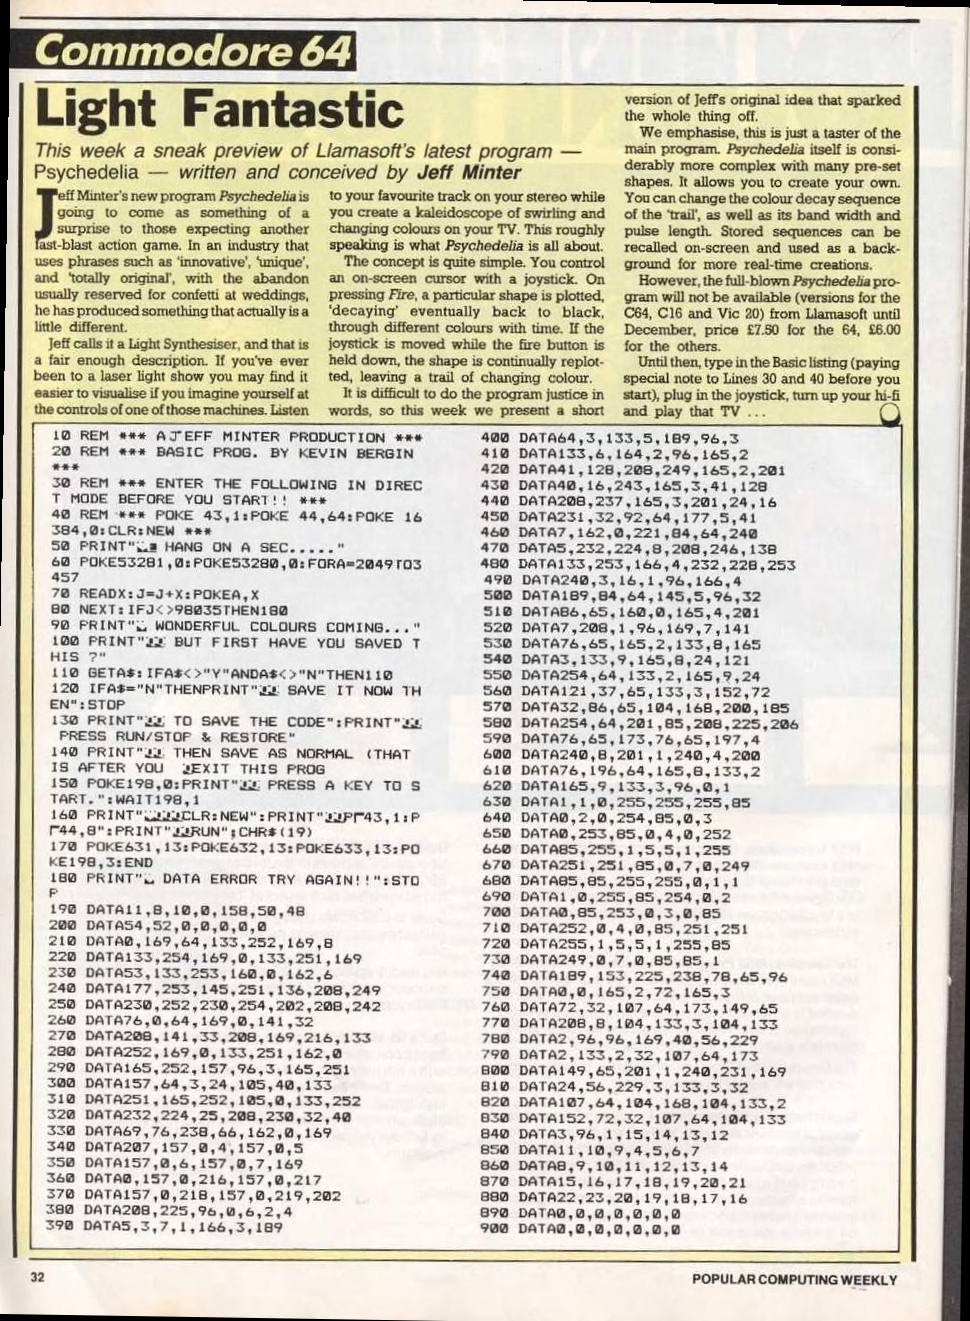
\includegraphics[width=12cm]{src/listing/PopularComputing_Weekly_Issue_1984-12-13_0031.jpg}}%
    \end{adjustbox}
\caption{You are expected to type all of this.}
\end{figure}
But this issue contained a saving grace that was guaranteed to have issues flying from the shelves ('Only 40p'). The cover needed only two
 words to communicate the delights awaiting: 'MINTER INSIDE'. On page 32 there was nothing less than a 'Jeff Minter special - preview of
\textit{Psychedelia}, Llamasoft's new release'. 1984 had been another busy year for Minter, he had completed two fairly large, but only
moderately successful, games in 'Sheep in Space' and 'Ancipital', as well as a clatter of lesser works. During the development of another
game, 'Mama Llama', he was struck by the inspiration for something completely novel. This was not a game but 'some kind of light synthesizer'.

\begin{definition}[Jeffrey Says]
\setlength{\intextsep}{0pt}%
\setlength{\columnsep}{3pt}%
\begin{wrapfigure}{l}{0.12\textwidth}

\includegraphics[width=\linewidth]{src/callout/psych.png} 
\end{wrapfigure}
\small
"I'd long
imagined some kind of light synthesiser I'd like to see at a gig or a party,
something with which you could visualise the very feel of a good piece of
music. I didn't imagine I could ever put such a concept successfully onto a
home micro, but one Sunday I got back from running and decided to have a
little tinker on my ‘64. An algorithm was in my head, it came from God
knows where, it was just there, complete. Maybe my subconscious made it.
Maybe my brain was leaking 3 months into the future. I coded it up,
assembled, SYSed in, picked up the joystick and blew my brains out."
\end{definition}

The rest of the game was completed in a two-week blitz in September 1984, and Minter immediately converted it to VIC20 and C16 while he was at it.
The listing in 'Popular Computing Weekly' was born of an eagerness to get the end result into people's hands. But in doing so, Minter
was handing over his work for a fairly modest consideration. 'Popular Computing Weekly' would have paid Jeff Minter a fee, probably in the range of £50-£100 (the customers meanwhile paid with their wits), but this hardly seems a fair exchange for a work that was the first of its kind.
'Psychedelia' after all was the first time anyone had written an interactive music visualizer for any kind of home computer. The only 
real predecessor of any kind was the 'Atari Video Music' released in 1977. THis was a physical appliance you plugged into your hi-fi and
your TV and which would display programmed visualizations with the ability to alter the display through physical switches and dials on the 
console itself.

\clearpage

\begin{figure}[H]
    \centering
    \begin{adjustbox}{width=12cm,center}
      \frame{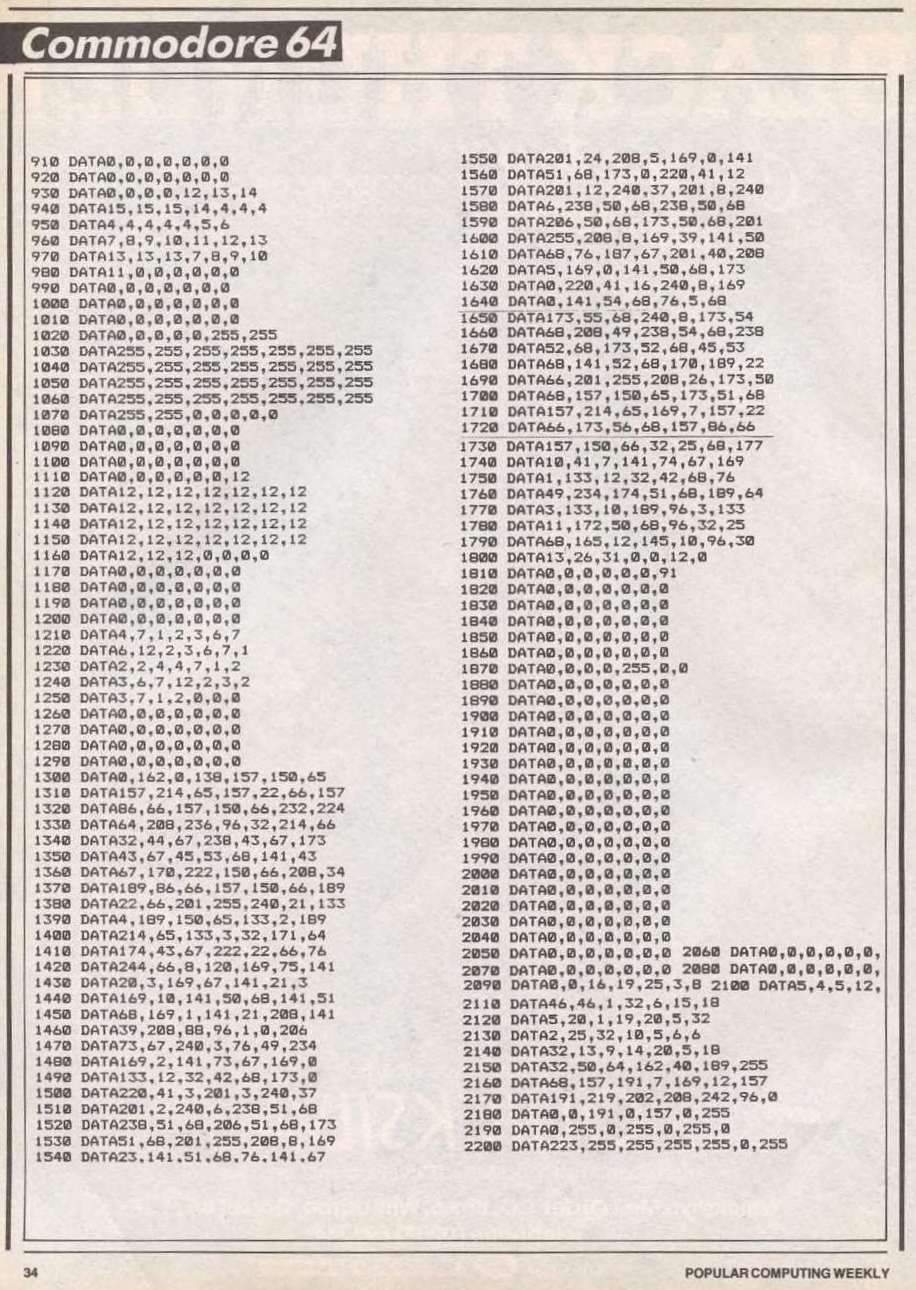
\includegraphics[width=12cm]{src/listing/PopularComputing_Weekly_Issue_1984-12-13_0033.jpg}}%
    \end{adjustbox}
\caption{And this.}
\end{figure}

Realizing this in software was something completely new and here was Minter giving it away more or less for free. Admittedly this was
a much reduced version of the commercial product. In order to fit it into a mere two pages of arduous number typing Minter had removed
nearly all the configurability that makes Psychedelia really compelling, but nevertheless the core of the game is in there, especially
the fundamental alogrithm that came to him while he was out for a jog that Sunday. Over the next few chapters we'll break down this
humble listing and get to understand it in all its parts. It will be the ideal way to understand how Psychedelia works in principle.
Once we have that we can look at all of the extras the final game came with and examine the workings of each individually.

For now though, let's place ourselves in the position of a spotty English teenager settling down in the days before Christmas to get
this thing up and running. Here we are, having fun: 

\begin{figure}[H]
    \centering
    \begin{adjustbox}{width=8cm,center}
      \frame{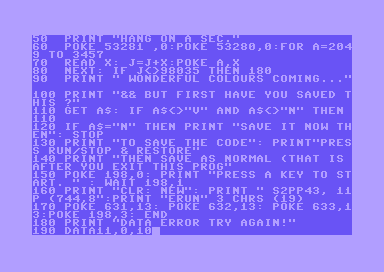
\includegraphics[width=12cm]{src/listing/typing.png}}%
    \end{adjustbox}
\caption*{Now the hell will start.}
\end{figure}

Above, we've got past the easy part - the almost-intelligble preamble that we can sort of understand.  Like all type-in listings of its day this consisted of a small BASIC program
that loads the raw machine code into memory. This isn't the juice of the program really.  

\lstset{style=C64BasicStyle}
\begin{lstlisting}
10  REM *** A JEFF MINTER PRODUCTION ***
20  REM *** BASIC PROG. BY KEVIN BERGIN ***
30  REM *** ENTER THE FOLLOWING IN DIREC T MODE BEFORE YOU START!! ***
40  REM *** POKE 43,1:POKE 44,44:POKE 16 384,0:CLR:NEW ***
50  PRINT "HANG ON A SEC."
60  POKE 53281 ,0:POKE 53280,0:FOR A=2049 TO 3457
70  READ X: J=J+X:POKE A,X
80  NEXT: IF J<>98035 THEN 180
90  PRINT " WONDERFUL COLOURS COMING..."
100 PRINT "&& BUT FIRST HAVE YOU SAVED THIS ?"
110 GET A$: IF A$<>"V" AND A$<>"N" THEN 110
120 IF A$="N" THEN PRINT "SAVE IT NOW THEN": STOP
130 PRINT "TO SAVE THE CODE": PRINT"PRESS RUN/STOP & RESTORE"
140 PRINT "THEN SAVE AS NORMAL (THAT IS AFTER YOU EXIT THIS PROG"
150 POKE 198,0: PRINT "PRESS A KEY TO START. " : WAIT 198,1
160 PRINT "CLR: NEW": PRINT " S2PP43, 11P (744,8":PRINT "ERUN" 3 CHRS (19)
170 POKE 631,13: POKE 632,13: POKE 633,13:POKE 198,3: END
180 PRINT "DATA ERROR TRY AGAIN!"
\end{lstlisting}

These lines perform the mundane task of reading in all of the numbers in the
rest of the listing and, once done, executing those numbers as a machine code
program. If you look closely you can see on line 80 there's a little sense-check in there too: all the numbers
we type in from the \icode{DATA} lines must add up to 98,035 or else we've made a mistake somewhere. If that happens
we get told \icode{DATA ERROR TRY AGAIN!}. As we will see a little later it was the grim fate of every child who
attempted to type in this listing to hit this error and never recover from it unless they performed some
inspired guesswork. This was a very cruel Christmas present.

But first lets understand what all these \icode{DATA} lines are all about. They are a long string of decimal
numbers each representing a byte of machine code. Minter wrote the game in 6502 Assembly Language, something
we will be seeing a lot of in future chapters, and using a program called an Assembler converted these
language instructions into a sequence of values between 0 and 255. This sequence forms the program itself.
When stored on disk or cassette it is usually termed a \icode{PRG} file because that is the conventional
suffix used for such files when naming them. In order to make it into a type-in-listing this binary file
has been converted into a simple list of decimal numbers, each one between 0 and 255. If you ever complete
typing in this listing, the numbers will get written to a location in the C64's memory and executed as 
machine code.

So what we're interested in is the assembly instructions that underlie that long list of numbers. Since 
6502 Assembly Language is so low-level this is surprisingly easy to do.


To give you an idea of how we get from raw numbers to an assembly program in practice I'll show you how
a little routine I call `PaintPixel` appears in the listing. Here it is as it appears in print:

\begin{figure}[H]
    \centering
    \begin{adjustbox}{width=7cm,center}
      \frame{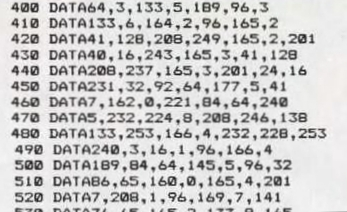
\includegraphics[width=12cm]{src/listing/PaintPixelShot.jpg}}%
    \end{adjustbox}
  \caption{These numbers contain a complete machine-code routine we've called \icode{PaintPixel}.}
\end{figure}

Our \icode{PaintPixel} routine starts towards the end of line \icode{410}:
\begin{lstlisting}
410 DATA                165,2
420 DATA 41,128,208,249,165,2,201
430 DATA 40,16,243,165,3,41,128
440 DATA 208,237,165,3,201,24,16
450 DATA 231,32,92,64,177,5,41
460 DATA 7,162,0,221,84,64,240
470 DATA 5,232,224,8,208,246,138
480 DATA 133,253,166,4,232,228,253
490 DATA 240,3,16,1,96,166,4
500 DATA 189,84,64,145,5,96   
\end{lstlisting}

Now let's look at the four stages we go through to transform this list of decimal numbers back into the original
assembly instruction. If you read left to right below, you can see the decimal values given in the listing translated to
hexadecimal, then to the meaning of those hexadecimal values in 6502 assembly language.

\lstset{style=6502Style}
\begin{lstlisting}[basicstyle=\ttfamily\scriptsize]
Decimal                   6502            Pretty  Assembly
Data          Hex         Assembly        with labels
-------       --------    ------------    ----------------------------------------
                                          PaintPixel                                       
165 2         A5 02       LDA $02           LDA pixelXPosition                               
41 128        29 80       AND #$80          AND #$80
208 249       D0 F9       BNE $089F         BNE ReturnEarly                                  
165 2         A5 02       LDA $02           LDA pixelXPosition                               
201 40        C9 28       CMP #$28          CMP #NUM_COLS                                    
16 243        10 F3       BPL $089F         BPL ReturnEarly                                  
165 3         A5 03       LDA $03           LDA pixelYPosition                               
41 128        29 80       AND #$80          AND #$80
208 237       D0 ED       BNE $089F         BNE ReturnEarly                                  
165 3         A5 03       LDA $03           LDA pixelYPosition                               
201 24        C9 18       CMP #$18          CMP #NUM_ROWS                                    
16 231        10 E7       BPL $089F         BPL ReturnEarly                                  
32 145 8      20 91 08    JSR $0891         JSR LoadXAndYPosition                            
177 5         B1 05       LDA ($05),Y       LDA (currentLineColorRamLoPtr),Y       
41 7          29 07       AND #$07          AND #COLOR_MAX                                   
162 0         A2 00       LDX #$00          LDX #$00                                         
                                          CheckPresetsLoop
221 137 8     DD 89 08    CMP $0889,X       CMP presetColorValuesArray,X             
240 5         F0 05       BEQ $08CB         BEQ MaybePaintPixel                                        
232           E8          INX               INX                                              
224 8         E0 08       CPX #$08          CPX #COLOR_MAX + 1                               
208 246       D0 F6       BNE $08C1         BNE CheckPresetsLoop                                        
                                          MaybePaintPixel   
138           8A          TXA               TXA                                      
133 253       85 FD       STA $FD           STA indexOfCurrentColor                          
166 4         A6 04       LDX $04           LDX colorIndexForCurrentPixel                    
232           E8          INX               INX                                              
228 253       E4 FD       CPX $FD           CPX indexOfCurrentColor                          
240 3         F0 03       BEQ $08D8         BEQ ActuallyPaintPixel                           
16 1          10 01       BPL $08D8         BPL ActuallyPaintPixel                           
96            60          RTS               RTS                                              
                                          ActuallyPaintPixel                               
166 4         A6 04       LDX $04           LDX colorIndexForCurrentPixel                    
189 137 8     BD 89 08    LDA $0889,X       LDA presetColorValuesArray,X                     
145 5         91 05       STA ($05),Y       STA (currentLineColorRamLoPtr),Y       
96            60          RTS               RTS                               
\end{lstlisting}

In the last column I've applied a final transformation where I invent names for each of the variables and
labels of loops and subroutines. This final bit of information exists only as raw numbers and addresses
in the machine code, so this last step is in a way pure invention on my part. When writing Psychedelia
there's no way Jeff Minter would have used such verbose names. They would have taken up too much space on
disk and too much real estate on the screen, not to mention that Camel-Casing was not possible on the computers
of the day which tended to display everything exclusively in an upper-case font. 

Comparing each column in the listing you quickly get a sense of what each decimal value maps to. For example, in
the very first line
\icode{165} maps to \icode{\$A5}, which maps to the \icode{LDA} instruction. This instruction loads the value
that follows it (\icode{\$02}) into the Accumulator register, one of three little pigeon-holes the 6502 CPU
has for storing values while doing its processing. Along with the \icode{X} and \icode{Y} registers, these little
pigeon-holes are used for nearly all temporary storage and indexing by 6502 assembly. If you want to add anything up,
compare one thing to another, or reference an array with an index number you are going to have to make use of one
or more of these registers.

But these kinds of details are all before us. For now, we are still stuck in our bedroom or on the carpet before
our living-room television typing in these bloody numbers. After an hour or two of careful dictation we think
we might be done. We've typed everything in, but towards the end we noticed something funny:

\begin{figure}[H]
    \centering
    \begin{adjustbox}{width=7cm,center}
      \frame{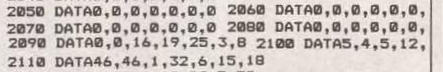
\includegraphics[width=12cm]{src/listing/clipped.jpg}}%
    \end{adjustbox}
  \caption{No more room on the page so just stick them in there beside those others.}
\end{figure}

This does not look right. There are numbers missing from the end of those lines! Anyone who didn't notice
this was doomed. There was no way of typing in what was on the page and passing the consistency check
built into the little BASIC program at the top of the listing. However, since we did notice it we can apply
a little enterprise and a little guesswork to retrieve the situation.

Here are the corrupted lines with an \icode{X} indicating each of our missing bytes:

\lstset{style=C64BasicStyle}
\begin{lstlisting}
2050 DATA 0,0,0,0,0,0,0 
2060 DATA 0,0,0,0,0,0,X
2070 DATA 0,0,0,0,0,0,0 
2080 DATA 0,0,0,0,0,0,X
2090 DATA 0,0,16,19,25,3,8 
2100 DATA 5,4,5,12,X,X,X
2110 DATA 46,46,1,32,6,15,18
\end{lstlisting}

Lines 2060 and 2080 are easy to guess: both are almost certainly \icode{0}. Why on earth the listing contains such
a long sequence of redundant zeroes is another matter. 

This leaves us with three bytes to fill. Is it too much to expect anyone to notice the pattern in these bytes that 
allows us to fill the gaps, least of all a bewildered teenager on their living room carpet? Can you? 


What if we do something as simple as assume each of these values refers to a letter in the alphabet? Doing so gives
us:

\begin{lstlisting}
16,19,25,3 ,8 ,5 ,4 ,5 ,12,X ,X ,X ,46,46,1 ,32,6 ,15,18
P ,S ,Y, C ,H ,E ,D ,E ,L ,X ,X ,X ,. ,. .A ,  ,F ,O , R
\end{lstlisting}

We are a genius. This must be text for the title screen or something. We can guess that the first two missing letters
are \icode{I} and \icode{A}, completing the word \icode{PSYCHEDELIA}. No prizes for that one.i However the final missing
letter could be either a space or a \icode{.}. Let's try a \icode{.}:

Our corrected listing reads:
\lstset{style=C64BasicStyle}
\begin{lstlisting}
2050 DATA 0,0,0,0,0,0,0 
2060 DATA 0,0,0,0,0,0,0
2070 DATA 0,0,0,0,0,0,0 
2080 DATA 0,0,0,0,0,0,0
2090 DATA 0,0,16,19,25,3,8 
2100 DATA 5,4,5,12,9,46
2110 DATA 46,46,1,32,6,15,18
\end{lstlisting}

We type 'RUN'. It works. My God, it actually works. 
\begin{figure}[H]
    \centering
    \begin{adjustbox}{width=12cm,center}
      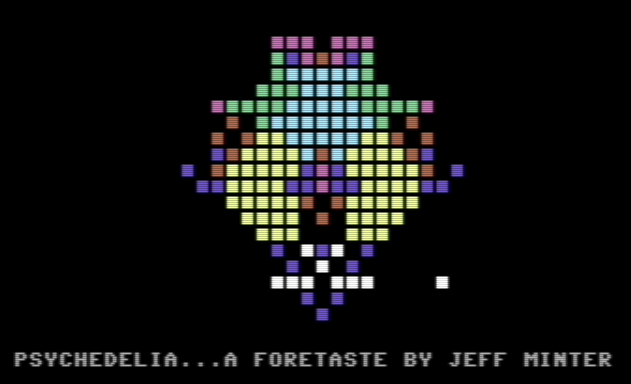
\includegraphics[width=12cm]{src/listing/itworks.png}%
    \end{adjustbox}
  \caption{The fruit of hours of pubescent toil.}
\end{figure}

The question this book asks is 'How does it work?'. For that, we will
need to pick this listing apart again and figure out its component parts. We will start 'in the middle', by looking at the
core algorithm that powers the psychedelic displays. This is the algorithm that came to Minter on his Sunday run.

